\chapter{Simulări și software folosit}
\label{chap:simulari}

\section{Dificultatea estimărilor parametrilor într-o rețea de apă}

Găsirea unui set de ecuații al cărei soluție să conducă la o estimare îndeajuns de bună pentru control este o condiție sine qua non pentru detecția unui defect și izolarea acestuia în cadrul nodurilor rețelei. Astfel după cum a fost expus în capitolul \ref{chap:intro} ecuațiile care guvernează relațiile intre viteza prin conducte și presiune dintr-un anumit punct sunt particularizări ale ecuațiilor Bernoulli-Euler sau Navier-Stokes. În cadrul unei rețele de apă a unui oraș, complexitatea rezolvării problemei crește semnificativ din varii motive precum:
\begin{itemize}
\item ansamblul de coduncte și noduri interconectate dă naștere unui sistem fizic greu de modelat matematic
\item parametrii care pot influența calitatea soluțiilor precum: tipul materialului conductei și al nodului, elevația fiecărui nod, rugozitatea fiecărei conducte și depunerile de pe aceasta
\item apariția unor factori exogeni care pot fi uneori greu de estimat - tiparul de utilizare al rețelei de către consumatori poate varia puternic
\item apariția defectelor precum scurgerile în proximitatea unui nod
\end{itemize}

Ținând cont de complexitatea problemei în regim dinamic pentru a putea obține o soluție de regim staționar a rețelei este necesar să ignorăm evenimentele imprevizibile precum apariția unei scurgeri sau variațiile bruște ale consumului.

Ecuațiile de regim staționar includ condiții de conservare fluxului de apă:

\begin{equation}
\label{Ecuația de conservare a rețelei de apă}
\sum\limits_{j=1}^{n} \mathbf B_{ij}\mathbf q_j=\mathbf d_i
\end{equation}

Unde $q_i$ reprezintă debitul prin fiecare conductă iar \textbf{B} reprezintă matricea de adiacență a rețelei la echilibru, definită astfel
\begin{equation}
\textbf{B}_{ij} = 
     \begin{cases}
       1, & \text{conducta j intră în nodul i}\\
       0, & \text{conducta j nu este conectată la nodul i} \\
       -1, & \text{conducta j iese din nodul i}\\ 
     \end{cases}
\end{equation}

Partea de estimare a diferenței de presiuni (în engl. "Head-Flow differential") între două noduri interconectate se face utilizând formula Hazen-Williams ;\cite{sanz2016demand}:
\begin{equation}
\label{debit_presiune}
\mathbf h_i-\mathbf h_j=\frac{10.67\cdot L_\ell}{C_\ell^{1.852}\cdot D_\ell^{4.87}}\cdot \mathbf q_\ell\cdot |\mathbf q_\ell|^{0.852}
\end{equation}

unde:
\begin{itemize}
\label{Hazen-Williams}
\item $\textbf{h}$ reprezintă presiunea - măsurată de obicei în metru coloană de apă
\item $C_l$  reprezintă coeficientul de rugozitate al conductei
\item $D_l$ reprezintă diametrul conductei
\item $L_l$ reprezintă lungimea conductei
\item $q_l$ reprezintă debitul
\end{itemize}

Din ecuația empirică \eqref{Hazen-Williams} termenul $R_{ij}=\frac{10.67\cdot L_\ell}{C_\ell^{1.852}\cdot D_\ell^{4.87}}$ reprezintă rezistența conductei $ij$ iar dual, putem obține conductivitatea conductei $G_{ij} = \frac{1}{R_{ij}}$

Având la dispoziție \eqref{Hazen-Williams} și \eqref{debit_presiune} putem exprima dependența debit presiune în regim staționar sub o formă matriceală compactă și cu o structură neliniară:

\begin{equation}
\mathbf B\mathbf G\left[\left(-\mathbf B^\top \mathbf h+\mathbf B_f^\top \mathbf h_f\right)\times \left|-\mathbf B^\top \mathbf h+\mathbf B_f^\top \mathbf h_f\right|^{-0.46}\right]=\mathbf d
\end{equation}

unde s-au luat în calcul și nodurile care au variații de presiune foarte mici - spre exemplu nodurile de tip tanc și  nodurile de tip rezervor - termenul $\mathbf B_f^\top \mathbf h_f$ reprezintă contribuția acestor noduri la starea de echilibru a rețelei.

Din cauza dificultății rezolvării unei ecuații matriceale neliniare, software-ul specializat trebuie să folosească diferite metode de optimizare ("Solver") pentru a putea obține o diferență cât mai mică între cazul estimat și rezultatul real al ecuației. Este important de reținut faptul că rezolvarea problemelor de programare neliniară cu constrângeri poate generea de fapt o problemă NP-completă, sau în unele cazuri chiar NP-dură ;\cite{karp1975computational}.

\section{Simulări folosind biblioteca EPANET}

	Dezvoltat la începutul anilor 90' de către USEPA (United States Environmental Protection Agency), EPANET a fost inițial privit ca un instrument pentru cercetare, acesta a devenit un standard de industrie la capitolul simulărilor software robuste pentru rețele de apă, foarte multe pachete software proprietare de simulare hidraulică se bazează masiv pe EPANET, diferențele apărând la design-ul interfeței grafice și a manipulării datelor. Aceast program de simulare oferă utilizatorului posibilitatea de a-și defini într-un mod interactiv o rețea de apă configurând tipul de nod, legătura între oricare două noduri și posibilitatea de a adăuga și elemente active în rețea, pompe. Pentru a simula utilizatorul trebuie să își definească pentru fiecare nod un anumit debit cerut de utilizatori, o elevație, și o legătură cu alte noduri. Simularea se va desfășura pe o perioadă de timp definită cu pasul de eșantionare cât mai convenabil ;\cite{rossman2000epanet}.
	
\begin{figure}[H]
\centering
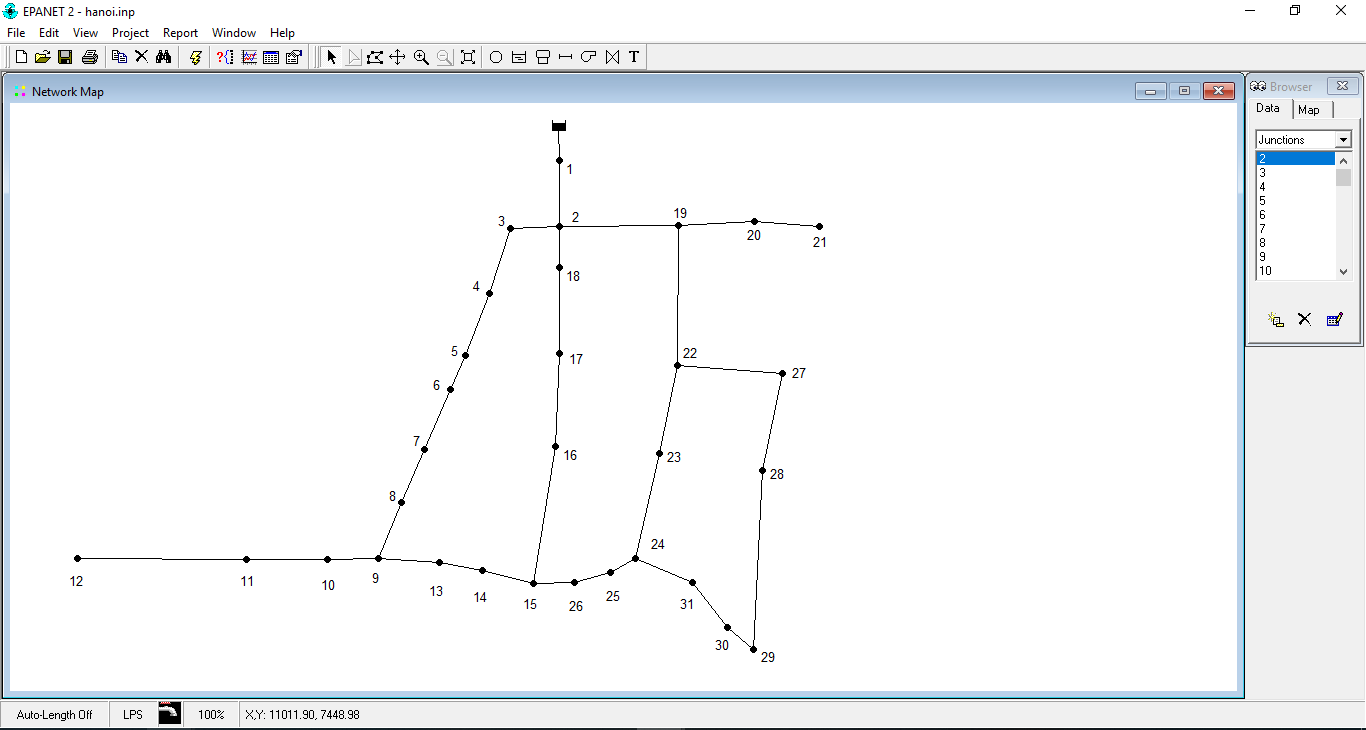
\includegraphics[width=0.75\textwidth]{pics/c2_pics/epanet_simulator.png}
\caption{Simulatorul EPANET}
\end{figure}

În urma execuției simulării EPANET va stoca toate datele în memorie și va putea reliza grafice și alte interogări complexe.

Modalitatea în care simulatorul EPANET reușește să obțină datele de simulare este prin implementarea eficientă a ecuațiilor  Hazen-Williams \eqref{Hazen-Williams} Darcy-Weisbach și Chezy-Manning, la fiecare perioadă de eșantionare algoritmul bazat de metoda gradientului rezolvă ecuațiile matriceale neliniare.